\subsubsubsubsection{Pedestrian crossing}
\begin{figure}[h]
\centering
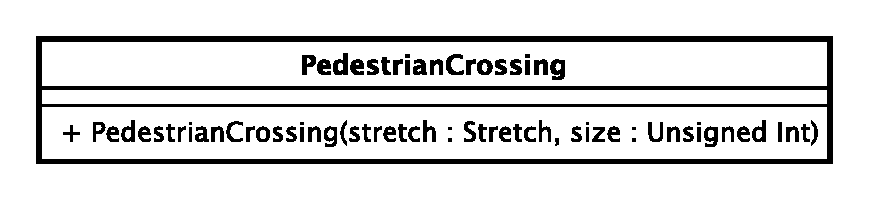
\includegraphics[scale=0.6,keepaspectratio]{images/solution/app/backend/pedestrian_crossing.eps}
\caption{\pReactiveComponentStretchDecoration::PedestrianCrossing}
\label{fig:sd-app-pedestrian_crossing}
\end{figure}
\FloatBarrier
\begin{itemize}
  \item \textbf{\descr} \\
    It represents the pedestrian crossing entity. Only pedestrians can tread this kind 
of crossing.
\item \textbf{\ops}
  \begin{itemize}
    \item[+] \texttt{PedestrianCrossing(stretch: Stretch, size: Unsigned Int)} \\
Creates a crossing for pedestrians with a specific size.
  	\end{itemize}
\end{itemize}
